% !TEX root =  main.tex
\chapter{The Classroom as a Binary Probabilistic Cellular Automata Model}
\hspace{\parindent} The classroom is a complex system that can be modeled as a probabilistic cellular automata. This chapter will discuss the classroom as a complex system and the probabilistic cellular automata model. The chapter will also discuss the implications of the model on the classroom and the teaching-learning process. (AI Generated Text)

Probably add objectives here???

\section{Cellular Automata and its use in modelling complex systems}

A two-dimensional (2D) rectangular cellular automata can be defined by a five-tuple \cite{arciaga2009experimental} + Reinier MS:

\begin{equation}
    \label{eq:CA definition}
    \text{CA} = \lbrace \mathcal{S,C,L,N,R} \rbrace
\end{equation}

where
\newlist{CAdef}{itemize}{1}
\newcommand\itemS{\item[$\mathcal{S}=$]}
\newcommand\itemC{\item[$\mathcal{C}=$]}
\newcommand\itemL{\item[$\mathcal{L}=$]}
\newcommand\itemN{\item[$\mathcal{N}=$]}
\newcommand\itemR{\item[$\mathcal{R}=$]}

\begin{CAdef}
    \itemS is the set of possible states that each cell can assume. The state $s$ can use any kind of representation such as the set of integers $\lbrace 0,\ldots,n-1\rbrace$ with $n$ as the total number of possible states.
    
    \itemC $\lbrace c = {i,j} \mid i \in \lbrace 1,2,3,\dots,L_1 \rbrace, j \in \lbrace 1,2,3,\dots,L_2\ \rbrace \text{s.t. } L_1 \times L_2 = N \rbrace$ is the set of identifiers for each cell in the automaton where $N$ is the total number of cells and $L_1$ and $L_2$ are the lengths of each side of the automaton space. The cells can then be identified by their position in the automaton $(i,j)$. So, the state of cell $c \in \mathcal{C}$ can be written as $s_c = s_{i,j} \in \mathcal{S}$
    
    \itemL defines the lattice neighborhood which is generally a mapping $f : \mathcal{C} \rightarrow C^M$ where $M$ is the number of neighbors of a cell $c \in \mathcal{C}$. Any given cell $c$ is mapped to another tuple of cells: $L_{i,j} = \lbrace (i-1,j-1), (i-1, j), (i-1, j+1), (i, j-1), \dots, (i,j)$. Where $r$ is the radius of the Moore neighborhood. We then say that $\mathcal{L}_{i,j}$ contains the set of neighboring cell for $c_{i,j}$.
    
    \itemN $\mathcal{S}^M$, the set of neighborhood states. Thus, $N_c = N_{i,j} \in \mathcal{N}$ such that each $\mathcal{N}$ is in the form of the $M$-tuple $\lbrace s_{i-1,j-1}, s_{i-1, j}, s_{i-1. j+1}, s_{i, j-1}, \dots, s_{i,j} \rbrace$.
    
    \itemR defines the set of rules implemented in the CA with $g : s_{i,j} \mid \mathcal{L} \rightarrow \mathcal{S}$ as the mapping of any neighborhood state $N_c$ to a new state $s'_{i,j}$ of the cell $c$. At the next time step, $s'_{i,j}$ replaces the original state $s_{i,j}$.
\end{CAdef}

% $\mathcal{S} = \lbrace 0,...,S-1 \rbrace$ is the set of representations of states each cell can take on.

% $\mathcal{C} = \lbrace c = {i,j} \mid i \in \lbrace 1,2,3,\dots,L_1 \rbrace, j \in \lbrace 1,2,3,\dots,L_2\ \rbrace \text{s.t. } L_1 \times L_2 = N \rbrace$ is the set of identifiers for each cell in the automaton where $N$ is the total number of cells and $L_1$ and $L_2$ are the lengths of each side of the automaton space. The cells can then be identified by their position in the automaton $(i,j)$. So, the state of cell $c \in \mathcal{C}$ can be written as $s_c = s_{i,j} \in \mathcal{S}$

% $\mathcal{L} =$ defines the lattice neighborhood which is generally a mapping $f : \mathcal{C} \rightarrow C^M$ where $M$ is the number of neighbors of a cell $c \in \mathcal{C}$. Any given cell $c$ is mapped to another tuple of cells: $L_{i,j} = \lbrace (i-1,j-1), (i-1, j), (i-1, j+1), (i, j-1), \dots, (i,j)$. Where $r$ is the radius of the Moore neighborhood. We then say that $\mathcal{L}_{i,j}$ contains the set of neighboring cell for $c_{i,j}$.

% $\mathcal{N} = \mathcal{S}^M$, the set of neighborhood states. Thus, $N_c = N_{i,j} \in \mathcal{N}$ such that each $\mathcal{N}$ is in the form of the $M$-tuple $\lbrace s_{i-1,j-1}, s_{i-1, j}, s_{i-1. j+1}, s_{i, j-1}, \dots, s_{i,j} \rbrace$.

% $\mathcal{R} =$ defines the set of rules implemented in the CA with $g : s_{i,j} \mid \mathcal{L} \rightarrow \mathcal{S}$ as the mapping of any neighborhood state $N_c$ to a new state $s'_{i,j}$ of the cell $c$. At the next time step, $s'_{i,j}$ replaces the original state $s_{i,j}$.

$\mathcal{N}$ can vary with the neighborhood structure and the boundary conditions of the automaton. The neighborhood structure dictates the shape the neighborhood in the lattice. Common neighborhood structures include the von Neumann (diamond) and Moore (square) neighborhoods. Boundary conditions dictate how the automaton treats cells at the egde of the lattice when determining the neighborhood. Common boundary conditions include toroidal, spherical, and fixed boundary conditions. 

$\mathcal{R}$ can also be affected by other factors such as whether the rules are deterministic or probabilistic and whether they are implemented synchronously or asynchronously. An automaton with deterministic rules will always produce the same output given the same input, while an automaton with probabilistic rules will produce different outputs given the same input. In Conway's Game of Life, a cell dies when it has three live neighbors, while a cell is born when it has two or three live neighbors. This is an example of a deterministic rule. An example of a probabilistic rule would be a cell dying with a probability of $0.25$ when it has three live neighbors. An automaton with synchronous rules will update all cells simultaneously, while an automaton with asynchronous rules will update cells one at a time. (something explanation something about sync vs async)


Due to the flexibility of cellular automata, they can be used to model a wide variety of complex systems. Cellular automata have been used to model physical systems such as fluid dynamics, biological systems such as the spread of diseases, and social systems such as traffic flow \cite{louis2018probabilistic}. Its discreteness and locality make it a good model for systems that are composed of many interacting parts. Thus, we have chosen to use a two-state probability cellular automata to simulate the learning process for students in the classroom


\section{PI as a Discrete Probabilistic CA Model}

We used a two-dimensional binary probabilistic cellular automata (PCA) model to simulate the learning process in a classroom. In this PCA model, each cell in the automaton represents a student and the state of each cell represents their aptitude $S=\lbrace\text{unlearned, learned}\rbrace=\lbrace 0,1 \rbrace$. We assign the neighborhood to be an outer-totalistic Moore neighborhood of radius $r=1$ and define the boundary conditions to be fixed wherein the grid does not wrap around itself and $s_{i,j} = 0$ for ${i,j \notin [1,L]}$. The rules of the automaton describes how the students learn from their neighbors based on three parameters. First (1), the learning rate $\lambda_{i,j}$ of student $c_{i,j}$ which describes how receptive they are to peer instruction. Secondly (2), the relative spatial factor $\rho_{i+\delta i, j+\delta j}$ which describes how likely it is to learn from the neighbor $c_{i+\delta i, j+\delta j}$ based solely on their relative position with respect to $c_{i,j}$. Lastly (3), the aptitude level of the neighbor $s_{i+\delta i, j+\delta j}$ which dictates whether student $c_{i,j}$ can learn from them. The probability for a student to learn in each time step is then determined by the following equation:

\begin{equation}
    \label{eq:BPCA PI learning probability}
        P_{ij} = 1 - \prod_{\forall \delta i, \delta j}{\lbrack1-(\lambda_{ij})(\rho_{i+\delta i, j+\delta j})(s_{i+\delta i, j+\delta j})}\rbrack
\end{equation}

where

$P_{i,j} \in [0,1]$ is the probability of $c_{i,j}$ to learn in each time step, 

$\lambda_{i,j} \in [0,1]$ is the learning rate of $c_{i,j}$ with values $\lambda_{i,j} = \lbrace \lambda_0 \pm \delta \lambda \rbrace$ where $\lambda_0 = 0.5$ and $\delta \lambda = \lbrace 0.1, 0.2, 0.3, 0.4 \rbrace$, 

$\rho_{i+\delta i, j+\delta j} \in [0,1]$ is the probability of $c_{i,j}$ to learn from their neighbors in seats $\lbrace c_{i+\delta i, j+\delta j} \forall \delta i, \delta j \in \lbrace -1,0,1 \rbrace \rbrace$ solely based from their relative positions with each other, and

$s_{i+\delta i, j+\delta j} = \lbrace\text{unlearned, learned}\rbrace=\lbrace 0,1 \rbrace$ are the neighbors aptitude level.

% \subsection*{spacing? idk}
\newpage
In the five-tuple form, the PCA model for the classroom can be written as:

\begin{CAdef}
\itemS $\lbrace \text{learned, unlearned} \rbrace = \lbrace 0, 1 \rbrace$

\itemC $\lbrace (1,1), (1,2), \dots, (1,L), (2, 1), (2,2), \dots, (2,L), \dots, (L,L)\rbrace$ where L is the length of the square classroom.

\itemL $f(c) \leftarrow \lbrack L_c = \lbrace (i+\delta i,j+\delta j) ~\forall~ (\delta i \land \delta j),  \delta i, \delta j \in \lbrace -1,0,1 \rbrace \rbrace $ as a mapping for outer-totalistic Moore neighborhood of radius $r=1$ with a fixed boundary condition.

\itemN $\lbrace 00000000, 00000001, \dots, 11111111 \rbrace$ such that the representation of the neighborhood state $N_c \in \mathcal{N}$ is equivalent to $N_c = \lbrace s_{i+\delta i, j+\delta j} \forall \delta i, \delta j \in \lbrace -1,0,1 \rbrace \rbrace$.

\itemR the probabilistic rule defined by equation \ref{eq:BPCA PI learning probability}.
\end{CAdef}

The numerical procedure is outlined in Figure \ref{fig:2DBPCA PI Flowchart}. Each simulation starts the classroom with four learned students $n_0 = 4$ placed in different seats in the classroom. 

\begin{figure}[h!]
    \centering
    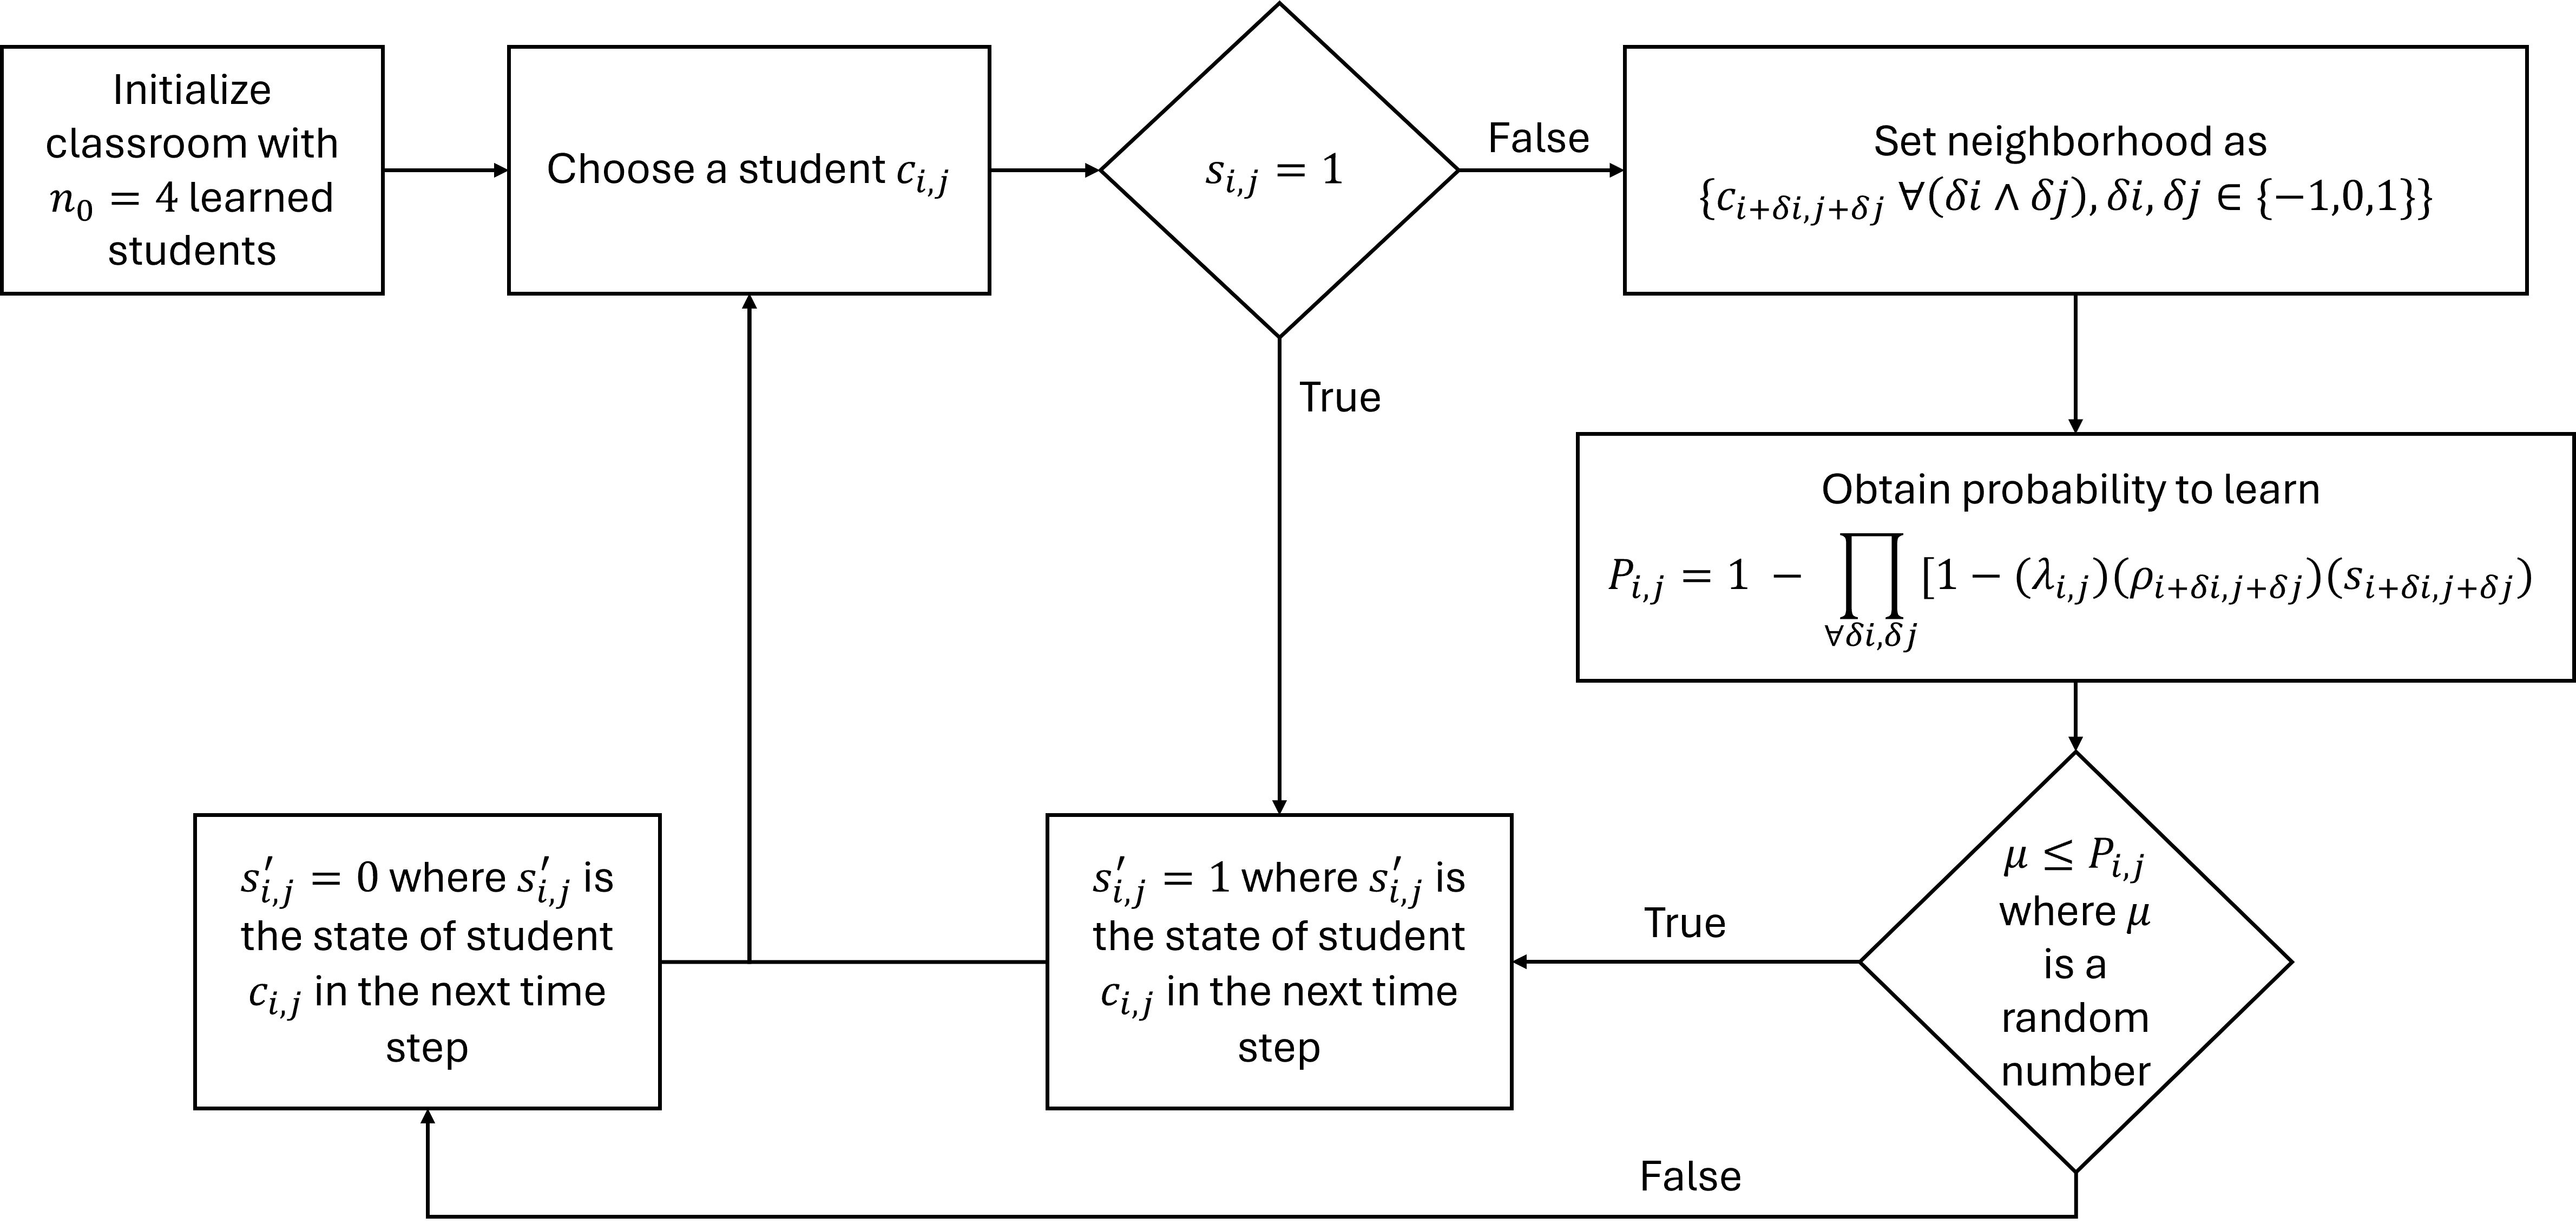
\includegraphics[width=0.8\textwidth]{figures/2DBPCA PI Flowchart.png}
    \caption[Peer instruction flowchart]{Numerical process for simulation of 2D BPCA for PI set-ups.}
    \label{fig:2DBPCA PI Flowchart}
\end{figure}

The seating arrangement (SA) were chosen from a previous study that showed that the SA can affect the learning process \cite{roxas2010seating}. These SA's are namely: inner corner, outer corner, center, and random. The SA configurations are shown in Figure \ref{fig:PI SAs}.

 \begin{figure}[h!]
    \centering
    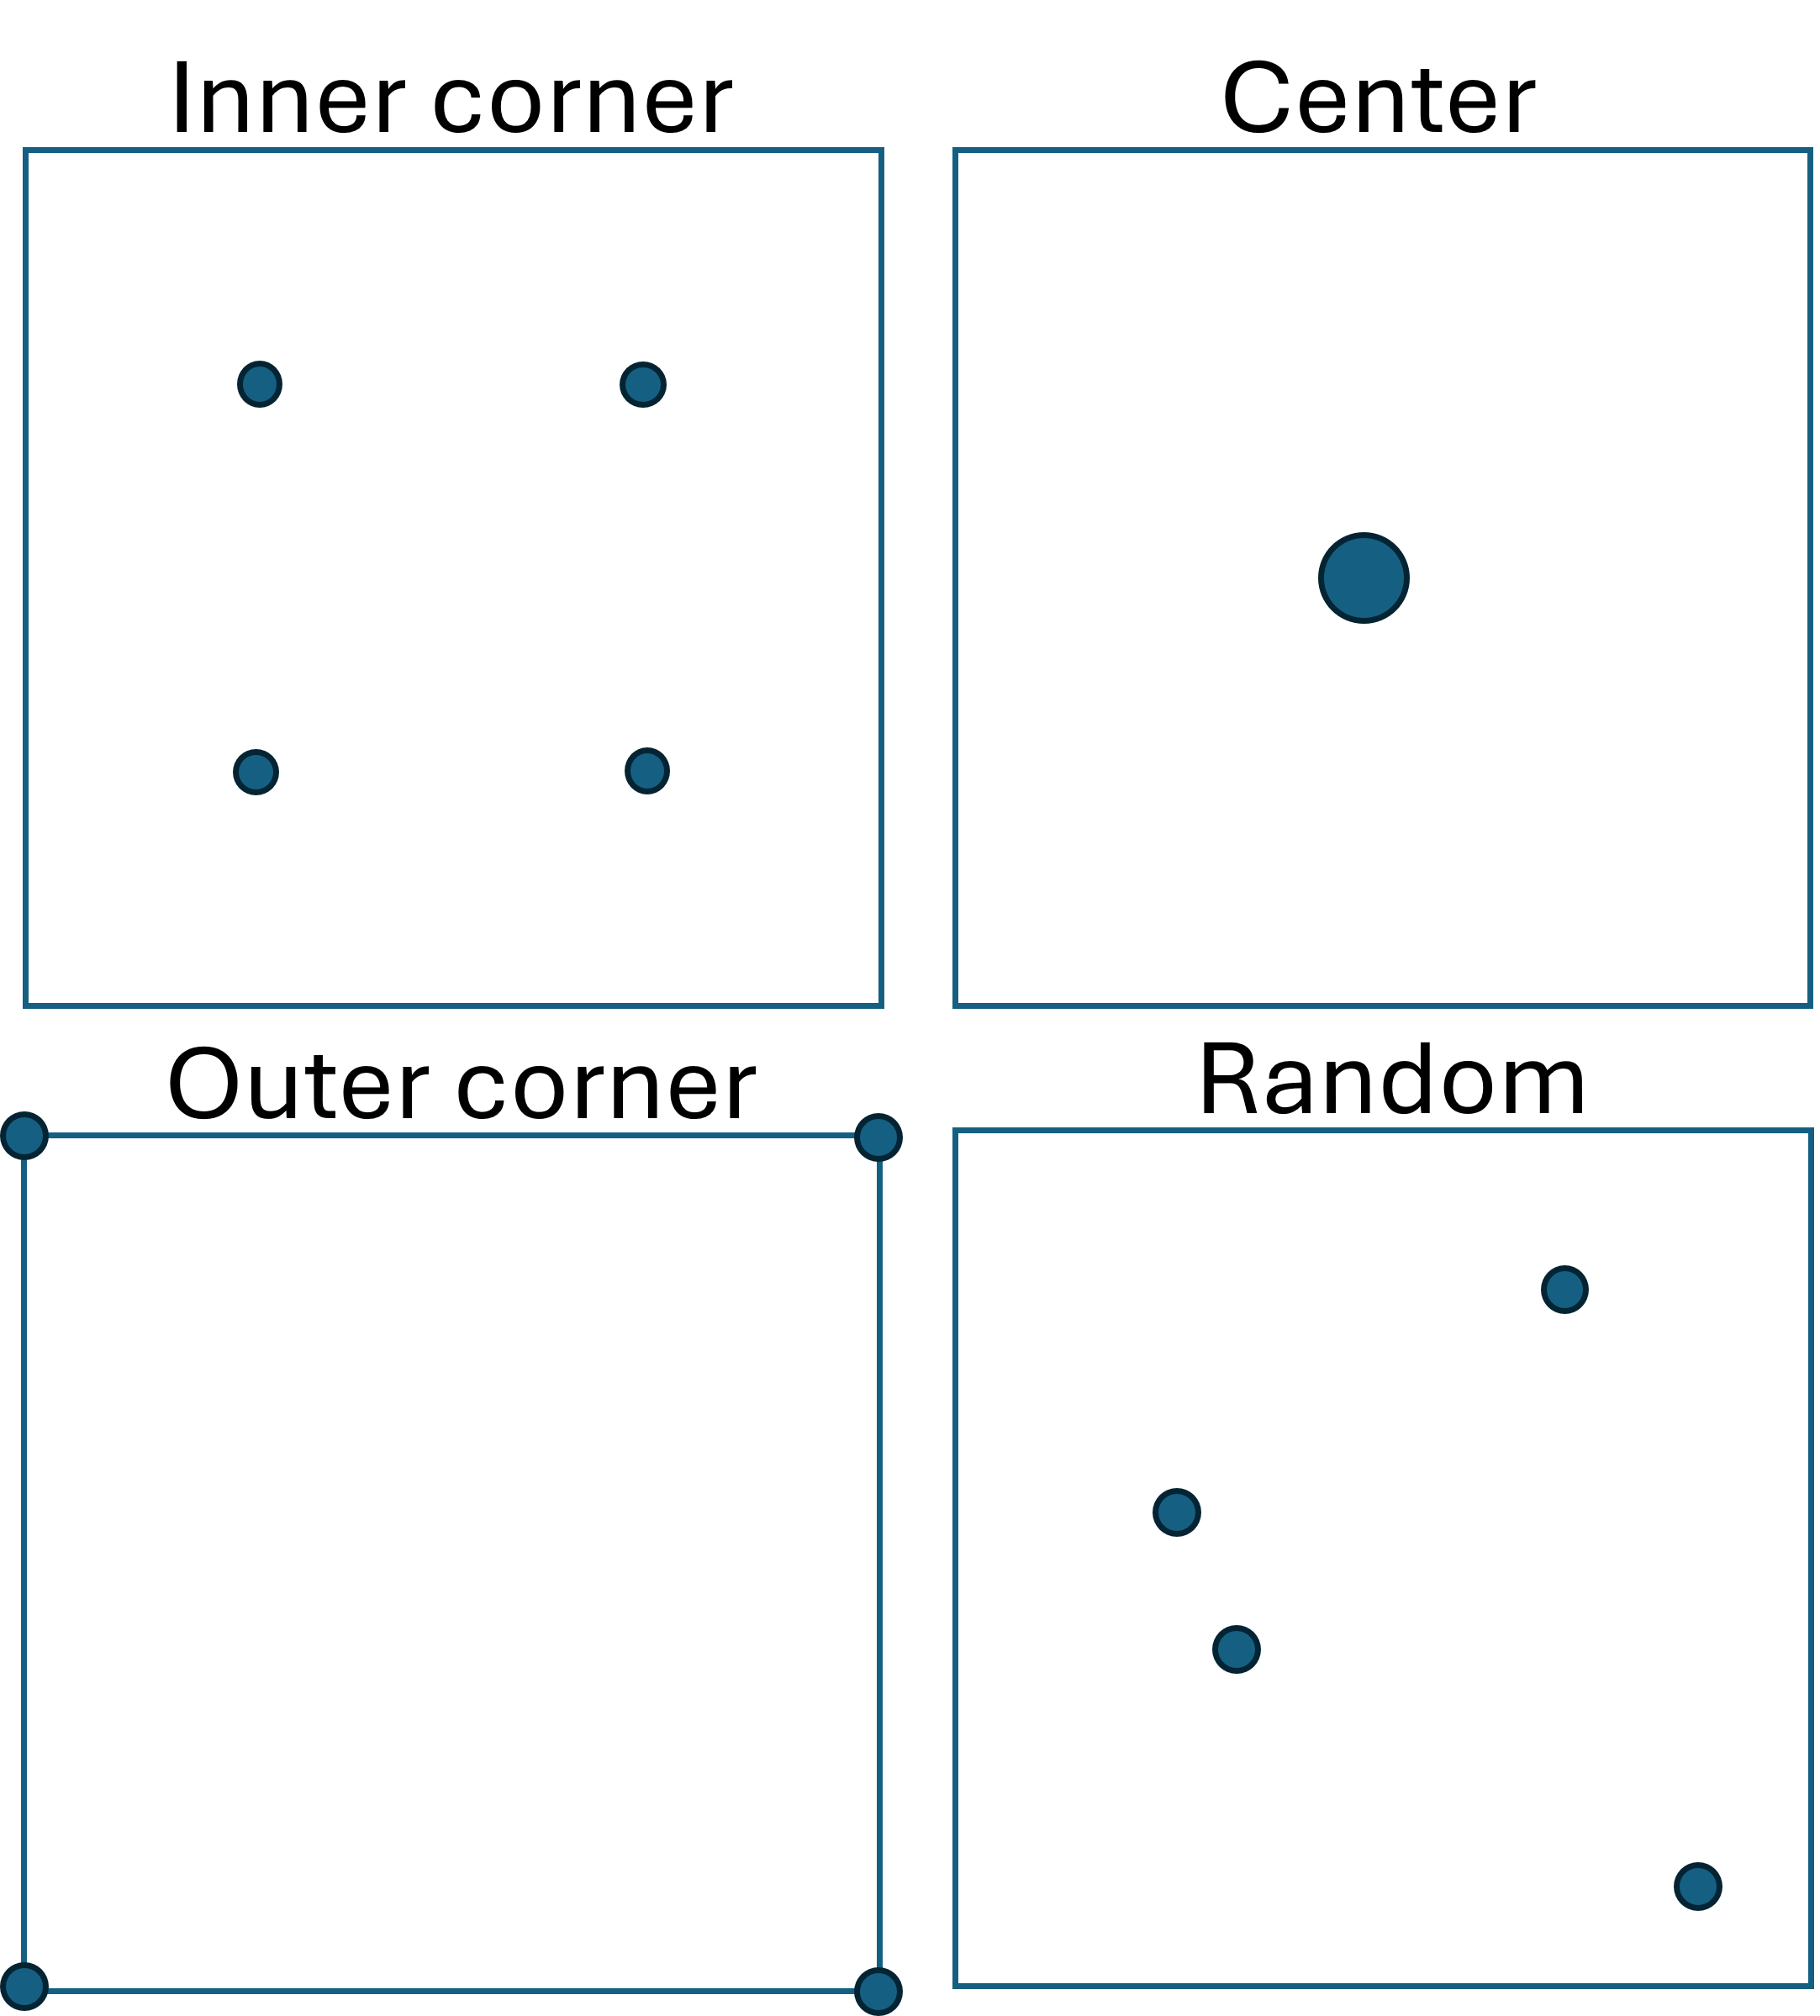
\includegraphics[width=0.5\textwidth]{figures/PI SAs.png}
    \caption[Peer instruction seating arrangements.]{ Peer instruction seating arrangements. Circles denote high aptitude students. The inner corner configuration places high aptitude students halfway between the center and the corner of the classroom. The outer corner configuration places high aptitude students at the corner of the classroom. The center configuration places high aptitude students in the center of the classroom. The random configuration places high aptitude students randomly throughout the classroom.}
    \label{fig:PI SAs}
 \end{figure}

 From the simulations, we compared both the average number time steps $\langle t_{max} \rangle$ it takes for all the students in the classroom to learn and the average learning rate $\langle m \rangle$ across different configurations over 5 independent runs. The learning rate for each trial was obtained by using a Levenberg-Marquardt algorithm to fit a power law ($y = ax^m$) to the fraction of learned students as a function of the generation number. We only considered the first $50\%$ of the data for the PI model or the first $25\%$ of the data for the traditional model. This truncation was done so that we only fit the part of the data before the finite size effect starts to affect the simulation.

\section{The binary probabilistic cellular automata model for a traditional classroom set up}
\begin{itemize}
    \item Governing equation:
    \begin{equation}
    \label{eq:BPCA traditional learning probability}
        P_{ij} = \lambda_0
    \end{equation}

    where:
    \subitem $P_{ij} \in [0,1]$ is the probability of the student seated in row $i$ and column $j$ to learn,
    \subitem $\lambda_0 \in [0,1]$ is the probability of the student $i,\space j$ to learn from the teacher

    \item Other relevant rules:
    \begin{enumerate}
        \item All students are unlearned at the start of the simulation.
        \item Simulation is considered done when all students are learned.
    \end{enumerate}
\end{itemize}

\section{Results: PI vs Traditional}
\begin{itemize}
    \item List of input and output parameters?
    \item $m$ vs $\lambda$ or $\rho_0$
    \item $t_{max}$ vs $\lambda$ or $\rho_0$
    \item $t_{max}$ vs $N$ for specific $\lambda$ or $\rho_0$
    \item Comparison between levels of homogeneity of learning rates
\end{itemize}

\section{Discussion/conclusions?}
\begin{enumerate}
    \item The traditional learning model is more scalable. Between the same $\rho$, the power law exponent $b$ is lower than its peer-to-peer counterpart.
    \item Inner corner configurations have higher b-values, while the traditional configurations have lower b-values.
    \item B-values generally increases with $\rho$ values
    \item Intersections where PI is more efficient occur at lower class sizes and lower $\rho$ values.
    
    \begin{itemize}
        \item In some class sizes, traditional and P2P approaches can become equally efficient depending on the learning rate $\rho$.
    \end{itemize}

    \item Similar finding with previous research \cite{lasry2008peer}: Students with less background knowledge learned as much with PI as students with more background knowledge with traditional instruction.

\end{enumerate}

    
